\documentclass[journal,12pt,onecolumn]{IEEEtran}
\usepackage{cite}
\usepackage{caption}
\usepackage{graphicx}
\usepackage{amsmath,amssymb,amsfonts,amsthm}
\usepackage{algorithmic}
\usepackage{graphicx}
\usepackage{textcomp}
\usepackage{xcolor}
\usepackage{tfrupee}
\usepackage{txfonts}
\usepackage{listings}
\usepackage{enumitem}
\usepackage{mathtools}
\usepackage{gensymb}
\usepackage{comment}
\usepackage[breaklinks=true]{hyperref}
\usepackage{tkz-euclide} 
\usepackage{listings}
\usepackage{gvv}
%\def\inputGnumericTable{}
\usepackage[latin1]{inputenc} 
\usetikzlibrary{arrows.meta, positioning}
\usepackage{xparse}
\usepackage{color}                                            
\usepackage{array}                                            
\usepackage{longtable}                                       
\usepackage{calc}                                             
\usepackage{multirow}
\usepackage{multicol}
\usepackage{hhline}                                           
\usepackage{ifthen}                                           
\usepackage{lscape}
\usepackage{tabularx}
\usepackage{array}
\usepackage{float}
\usepackage{marvosym}
\usepackage{float}
%\newcommand{\define}{\stackrel{\triangle}{=}}
\theoremstyle{remark}
\usepackage{circuitikz}
\captionsetup{justification=centering}
\usepackage{tikz}

\title{Matrices in Geometry 10.5.5}
\author{EE25BTECH11037 - Divyansh}
\begin{document}
\vspace{3cm}
\maketitle
{\let\newpage\relax\maketitle}
\textbf{Question: }
Construct a tangent to a circle of radius $4cm$ from a point on the concentric circle of radius $6cm$ and measure its length. Also verify the measurement by actual calculation.
\vspace{2mm}


\textbf{Solution:}
Let center be the origin. Then the circle with radius $4 \ cm$ is
\begin{align}
    \vec{C} \ : \ \vec{x}^{\top}\vec{V}\vec{x} + 2\vec{u}^{\top}\vec{x} + f=0 \ ; \ \vec{V}=\myvec{1&0\\0&1} \ , \ \vec{u}=\myvec{0\\0} \ , \ f=-16
\end{align}
Let the external point from which the tangent is drawn be $\vec{h}=\myvec{6\\0}$.\\
Let us calculate the matrix $\Sigma$
\begin{align}
    \Sigma=\brak{\vec{V}\vec{h} + \vec{u}}\brak{\vec{V}\vec{h} + \vec{u}}^{\top} - g\brak{\vec{h}}\vec{V}\\
    g\brak{\vec{h}}=\vec{h}^{\top}\vec{V}\vec{h} + 2\vec{u}^{\top}\vec{h} + f =\norm{\vec{h}}^2 +f =36-16 =20\\
    \Sigma = \vec{h}\vec{h}^{\top} - g\brak{\vec{h}}\vec{V}=\myvec{6 \\ 0}\myvec{6 & 0} - 20\myvec{ 1& 0 \\ 0 &1}\\
    \implies \Sigma=\myvec{16 & 0 \\ 0 & -20}
\end{align}
The eigenvalues of the matrix $\Sigma$ are clearly $\lambda_1=16$ and $\lambda_2=-20$\\
The normalized eigenvectors form the matrix $\vec{P}$.
\begin{align}
    \vec{P}=\myvec{1 & 0\\0&1}
\end{align}
The direction vectors of the two tangents are
\begin{align}
    \vec{m}=\vec{P}\myvec{\abs{\lambda_2} \\ \pm\sqrt{\abs{\lambda_1}}}=\myvec{2\sqrt{5} \\ \pm 4}
\end{align}
The length of the tangent is given by
\begin{align}
    \norm{\vec{T}-\vec{h}}=\abs{\mu} \norm{\vec{m}} \ , \ \brak{\text{$\mu$ is a parameter}}\\
    \mu= -\dfrac{\vec{m}^{\top} \brak{\vec{V}\vec{h} + \vec{u}}}{\norm{\vec{m}}^2} =-\dfrac{\myvec{2\sqrt{5} & 4} \myvec{6\\0}}{\norm{\myvec{2\sqrt{5} \\ 4}}^2}=-\dfrac{\sqrt{5}}{3}\\
    \therefore \norm{\vec{T}-\vec{h}}=\dfrac{\sqrt{5}}{3} \times 6 = 2\sqrt{5} \approx 4.47 \ cm
\end{align}
From the figure given below, we can verify that both lengths are equal and equal to $4.47$ cm.
\begin{figure}
    \centering
    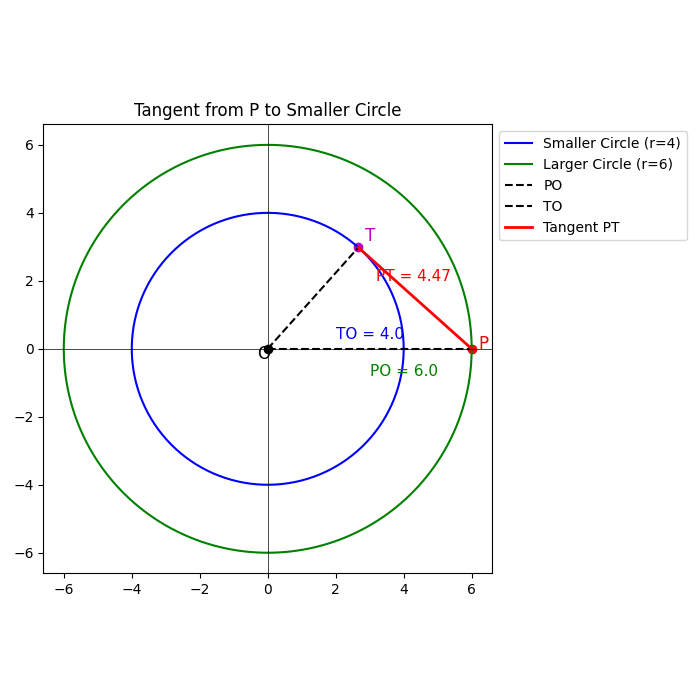
\includegraphics[width=1\columnwidth]{figs/1.png}
    \caption{Graph for 10.5.5}
    \label{fig:placeholder}
\end{figure}
\end{document}

